\subsection{Map}\label{ssec:map}
The map data type stores 2D spatial data, such as images of the Sun and 
inner heliosphere. It provides: a wrapper around a \texttt{numpy} data array, 
the images associated spatial coordinates, and other metadata. The \texttt{Map} 
class provides methods for typical operations on 2D data, such as rotation and 
re-sampling, as well as visualisation functionality.
The \texttt{Map} class also provides a convenient interface for loading data 
from a variety of sources, including a FITS file as shown in 
Listing~\ref{code:aia_1}.

The architecture of the map subpackage consists of a template map called
\texttt{GenericMap}, which is a subclass of \texttt{astropy.nddata.NDData}. 
\texttt{NDData} is a generic wrapper around a \texttt{numpy.ndarray} with a 
\texttt{meta} attribute to store metadata.
As \texttt{NDData} is currently still in development, \texttt{GenericMap} does 
not yet make full use of its capabilities, but this inheritance structure 
provides for future integration with \texttt{astropy}. In order to provide 
instrument- or detector-specific integration, \texttt{GenericMap} is designed
to be subclassed. Each subclass of \texttt{GenericMap} can register 
with the \texttt{Map} creation factory, which will then automatically return an instance
of the specific \texttt{GenericMap} subclass dependent upon the data provided. 
SunPy v0.4 has \texttt{GenericMap} specialisations for the following 
instruments: 
\textit{Yohkoh}/SXT, \textit{SOHO}/EIT and LASCO, \textit{RHESSI}, 
\textit{STEREO}/EUVI and COR, \textit{Hinode}/XRT,
\textit{PROBA2}/SWAP, \textit{SDO}/AIA and HMI, 
and \textit{IRIS} SJI frames. 
                        
The \texttt{Map} class stores all of the metadata retrieved from the header of
the image file in the \texttt{meta} attribute and provides convenience 
properties for commonly accessed metadata: e.g., \texttt{instrument}, 
\texttt{wavelength} or \texttt{coordinate\_system}. 
Listing \ref{code:aia_1} demonstrates the quick-look functionality of 
\texttt{Map}.

\begin{listing}[H]
\begin{minted}[bgcolor=bg]{pycon}
>>> import sunpy.map
>>> aiamap = sunpy.map.Map("aia_file.fits")
>>> smap = aiamap.submap([-1200, -200], [-1000, -0])
>>> smap.peek(draw_grid=True)
\end{minted}
\begin{center}
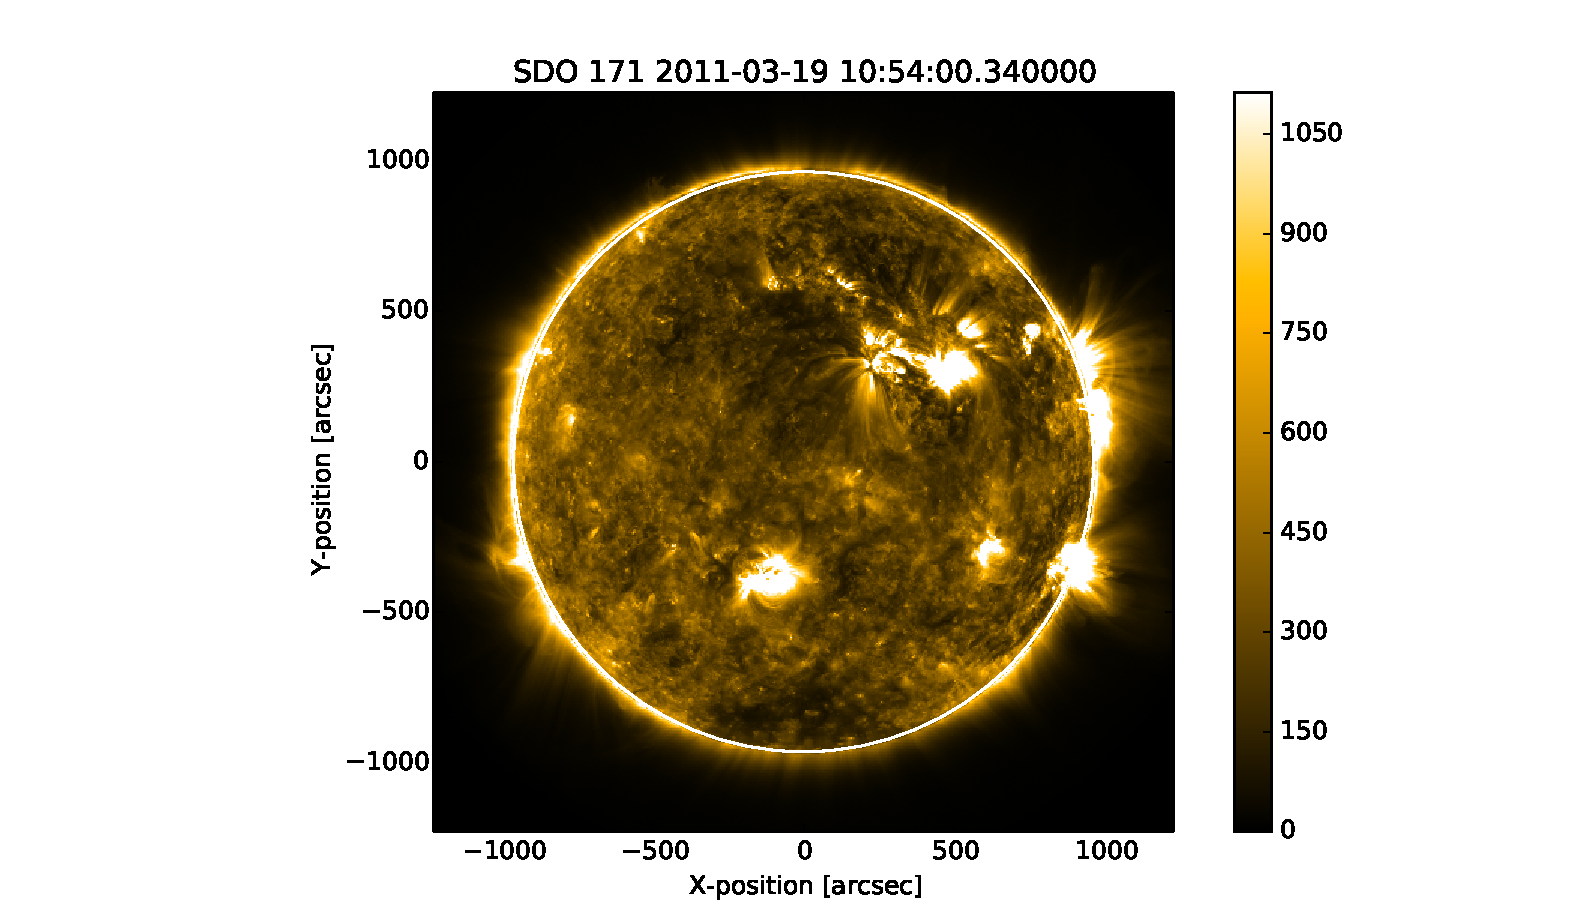
\includegraphics[width=0.8\columnwidth]{aia_map_example}
\end{center}
\caption{Example of the \texttt{AIAMap} specialisation of 
\texttt{GenericMap}. The map is created from an \textit{SDO}/AIA FITS file, a cutout
of the map is created, and then a quick-view plot is created with lines of heliographic longitude and latitude over-plotted.}
\label{code:aia_1}
\end{listing}

In addition to the data-type classes, the \texttt{map} subpackage provides two 
collection classes, \texttt{CompositeMap} and \texttt{MapCube}, for 
spatially and temporally aligned data respectively.
\texttt{CompositeMap} provides methods for overlaying spatially aligned 
data, with support for visualisation of images and contour lines overlaid 
upon each other.
\texttt{MapCube} provides methods for animation of its series of \texttt{Map} 
objects. Listings~\ref{code:compmap_1} and \ref{code:mapcube_1} show how to 
interact with these classes.

\begin{listing}[H]
\begin{minted}[bgcolor=bg]{pycon}
>>> import sunpy.map
>>> import matplotlib.pyplot as plt
>>> compmap = sunpy.map.Map("aia_1600_image.fits", "RHESSI_image.fits", 
...                         composite=True)
>>> compmap.set_levels(1, range(0, 50, 5), percent=True)
>>> compmap.set_colors(1, "Reds_r")
#Plot the result and crop
>>> ax = plt.subplot()
>>> compmap.plot()
>>> ax.axis([200, 600, -600, -200])
>>> plt.show()
\end{minted}
\begin{center}
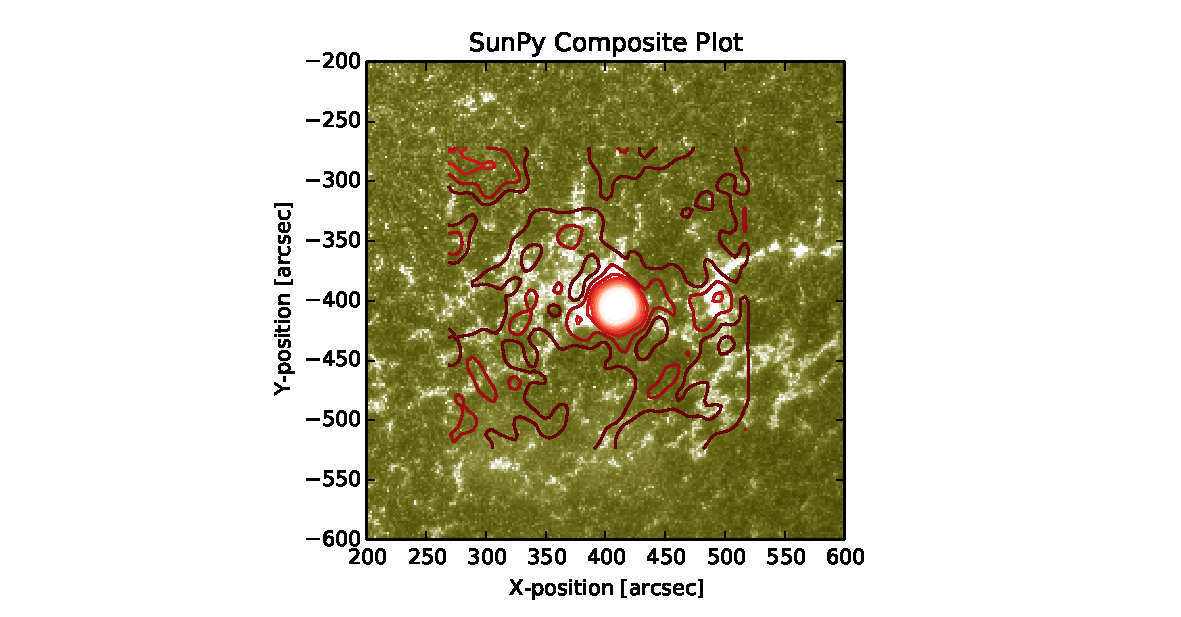
\includegraphics[width=0.8\columnwidth]{comp_map_example}
\end{center}
\caption{Example showing the functionality of \texttt{CompositeMap}, with RHESSI data composited
on top of \textit{SDO}/AIA data. The \texttt{CompositeMap} is plotted using the integration with the \texttt{matplotlib.pyplot} interface.}
\label{code:compmap_1}
\end{listing}

\begin{listing}[H]
\begin{minted}[bgcolor=bg]{pycon}
>>> import sunpy.map
>>> cubemap = sunpy.map.Map("aia_lev1_171a_2014_01*fits", cube=True)
>>> cubemap.peek()
\end{minted}
\begin{center}
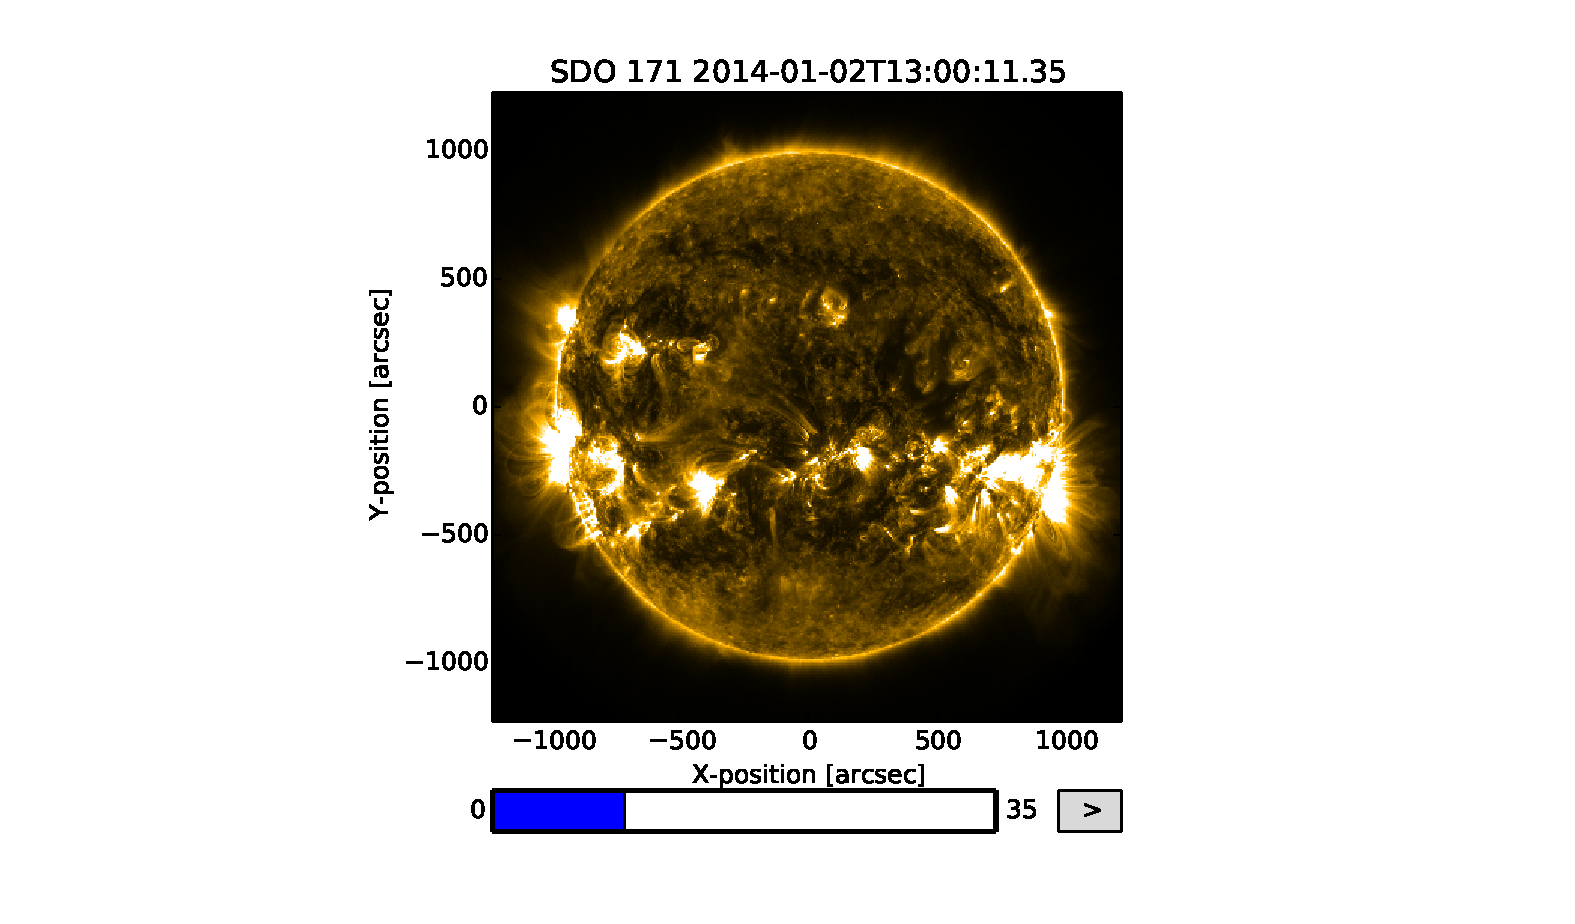
\includegraphics[width=0.8\columnwidth]{aia_cube_controls}
\end{center}
\caption{Example showing the creation of a \texttt{MapCube} from a list of files. The 
resultant plot makes use of \texttt{matplotlib}'s interactive widgets to allow scrolling 
through the \texttt{MapCube}.}
\label{code:mapcube_1}
\end{listing}